% !TeX program = arara -p generate_examples % | txs:///view-log | txs:///view-pdf "?am).pdf"
\documentclass{standalone}
\usepackage{tikzducks,tikzlings}

\begin{document}

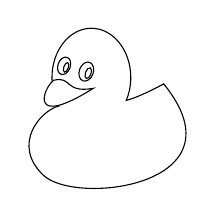
\begin{tikzpicture}

  \path (0.1,0.08) rectangle (2.12,2.14);

  \draw[overlay,cm={{0.75,0.0,0.0,-0.75,(0.0,2.2)}}] (1.1800,0.0899) .. controls (0.8116,0.0899) and (0.5129,0.4633) .. (0.5129,0.9238) .. controls (0.5129,1.1027) and (0.5584,1.2680) .. (0.6351,1.4038) .. controls (0.3064,1.4888) and (-0.1718,2.0636) .. (0.3648,2.5769) .. controls (0.9185,3.1052) and (3.7990,2.7516) .. (2.4048,1.0319) .. controls (2.1085,1.1911) and (1.9129,1.2733) .. (1.7701,1.3123) .. controls (1.8191,1.1963) and (1.8471,1.0642) .. (1.8471,0.9238) .. controls (1.8471,0.4633) and (1.5485,0.0899) .. (1.1800,0.0899) -- cycle;
  \draw[fill=white] \duckpathbill;
  \draw[rotate=-20] (0.23,1.7675) ellipse[x radius=0.0893, y radius=0.125];
  \draw[rotate=-20] (0.26,1.7575) ellipse[x radius=0.0357, y radius=0.0714];
  \draw[rotate=-20] (-0.06,1.74) ellipse[x radius=0.0786, y radius=0.1143];
  \draw[ rotate=-20] (-0.03,1.73) ellipse[x radius=0.0286, y radius=0.0643];
  
\end{tikzpicture}

\end{document}